\item A viga tem uma massa de $\SI{750}{\kilogram}$ e está sendo levantada para uma posição vertical puxando-se muito devagar sua extremidade inferior $A$. Se a corda arrebenta quando $\theta=\SI{60}{^{\circ}}$, e a viga está essencialmente em repouso, determine a velocidade de $A$ no instante que a corda $BC$ torna-se vertical. Despreze o atrito e a massa das cordas e trate a viga como uma barra fina.

\begin{flushright}
	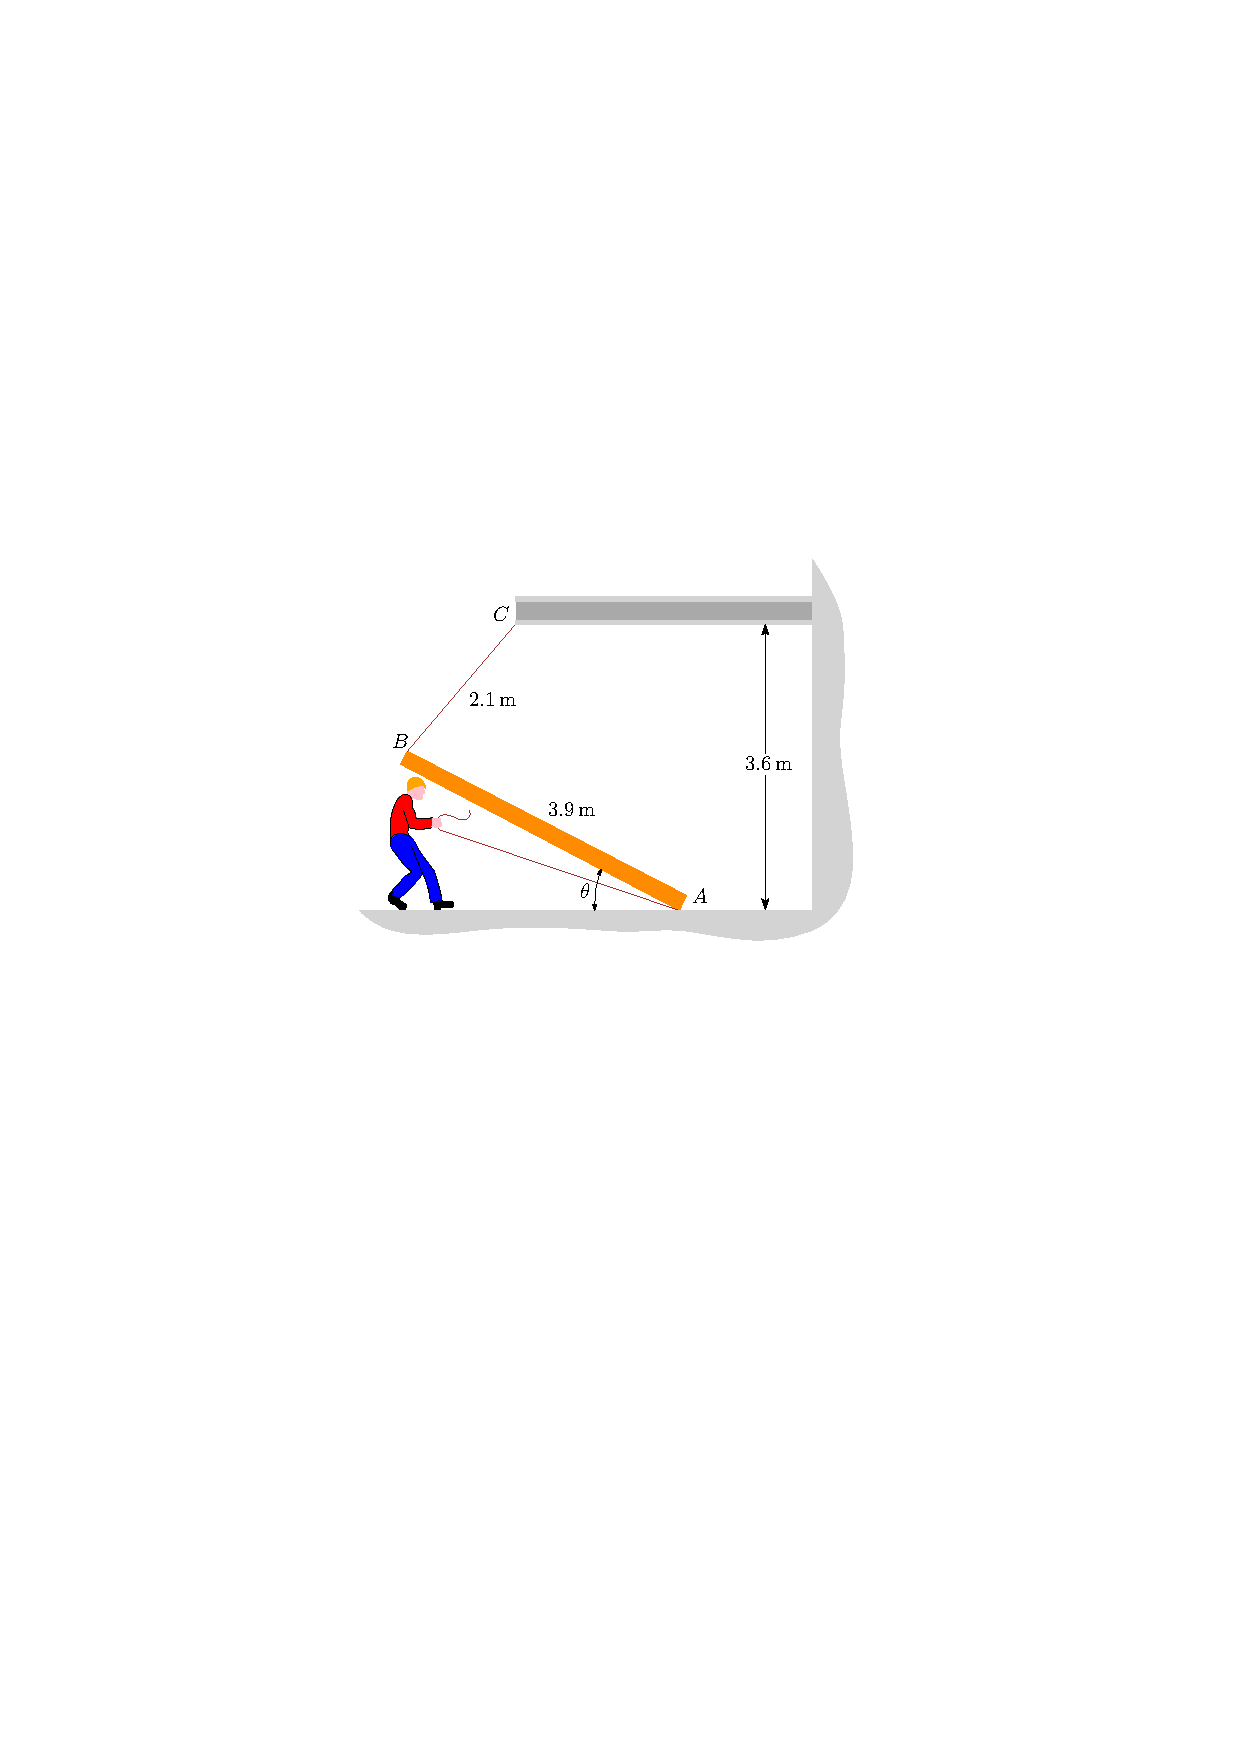
\includegraphics[scale=1.25]{../../images/draw_4_2}
\end{flushright}
